% Created by tikzDevice version 0.12.6 on 2026-05-17 11:17:49
% !TEX encoding = UTF-8 Unicode
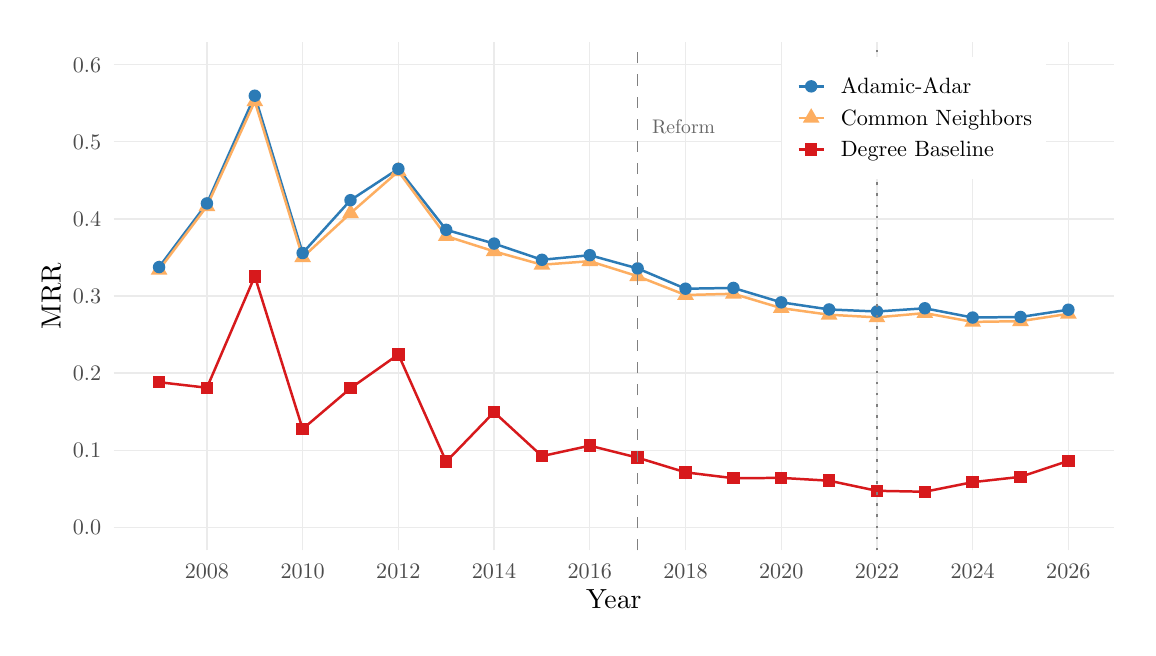
\begin{tikzpicture}[x=1pt,y=1pt]
\definecolor{fillColor}{RGB}{255,255,255}
\path[use as bounding box,fill=fillColor,fill opacity=0.00] (0,0) rectangle (397.48,216.81);
\begin{scope}
\path[clip] (  0.00,  0.00) rectangle (397.48,216.81);
\definecolor{fillColor}{RGB}{255,255,255}

\path[fill=fillColor] ( -0.00,  0.00) rectangle (397.48,216.81);
\end{scope}
\begin{scope}
\path[clip] ( 31.05, 27.90) rectangle (392.48,211.81);
\definecolor{drawColor}{gray}{0.92}

\path[draw=drawColor,line width= 0.5pt,line join=round] ( 31.05, 36.26) --
	(392.48, 36.26);

\path[draw=drawColor,line width= 0.5pt,line join=round] ( 31.05, 64.12) --
	(392.48, 64.12);

\path[draw=drawColor,line width= 0.5pt,line join=round] ( 31.05, 91.99) --
	(392.48, 91.99);

\path[draw=drawColor,line width= 0.5pt,line join=round] ( 31.05,119.85) --
	(392.48,119.85);

\path[draw=drawColor,line width= 0.5pt,line join=round] ( 31.05,147.72) --
	(392.48,147.72);

\path[draw=drawColor,line width= 0.5pt,line join=round] ( 31.05,175.58) --
	(392.48,175.58);

\path[draw=drawColor,line width= 0.5pt,line join=round] ( 31.05,203.45) --
	(392.48,203.45);

\path[draw=drawColor,line width= 0.5pt,line join=round] ( 64.77, 27.90) --
	( 64.77,211.81);

\path[draw=drawColor,line width= 0.5pt,line join=round] ( 99.36, 27.90) --
	( 99.36,211.81);

\path[draw=drawColor,line width= 0.5pt,line join=round] (133.95, 27.90) --
	(133.95,211.81);

\path[draw=drawColor,line width= 0.5pt,line join=round] (168.53, 27.90) --
	(168.53,211.81);

\path[draw=drawColor,line width= 0.5pt,line join=round] (203.12, 27.90) --
	(203.12,211.81);

\path[draw=drawColor,line width= 0.5pt,line join=round] (237.71, 27.90) --
	(237.71,211.81);

\path[draw=drawColor,line width= 0.5pt,line join=round] (272.30, 27.90) --
	(272.30,211.81);

\path[draw=drawColor,line width= 0.5pt,line join=round] (306.88, 27.90) --
	(306.88,211.81);

\path[draw=drawColor,line width= 0.5pt,line join=round] (341.47, 27.90) --
	(341.47,211.81);

\path[draw=drawColor,line width= 0.5pt,line join=round] (376.06, 27.90) --
	(376.06,211.81);
\definecolor{drawColor}{RGB}{44,123,182}

\path[draw=drawColor,line width= 0.9pt,line join=round] ( 47.48,130.30) --
	( 64.77,153.31) --
	( 82.07,192.22) --
	( 99.36,135.38) --
	(116.65,154.47) --
	(133.95,165.80) --
	(151.24,143.76) --
	(168.53,138.79) --
	(185.83,132.93) --
	(203.12,134.59) --
	(220.41,129.81) --
	(237.71,122.48) --
	(255.00,122.76) --
	(272.30,117.56) --
	(289.59,114.99) --
	(306.88,114.24) --
	(324.18,115.41) --
	(341.47,112.06) --
	(358.76,112.27) --
	(376.06,114.89);
\definecolor{drawColor}{RGB}{253,174,97}

\path[draw=drawColor,line width= 0.9pt,line join=round] ( 47.48,129.31) --
	( 64.77,152.30) --
	( 82.07,190.19) --
	( 99.36,133.83) --
	(116.65,149.76) --
	(133.95,164.90) --
	(151.24,141.48) --
	(168.53,135.98) --
	(185.83,131.15) --
	(203.12,132.42) --
	(220.41,126.99) --
	(237.71,120.20) --
	(255.00,120.65) --
	(272.30,115.47) --
	(289.59,113.08) --
	(306.88,112.13) --
	(324.18,113.67) --
	(341.47,110.49) --
	(358.76,110.75) --
	(376.06,113.41);
\definecolor{drawColor}{RGB}{215,25,28}

\path[draw=drawColor,line width= 0.9pt,line join=round] ( 47.48, 88.70) --
	( 64.77, 86.70) --
	( 82.07,126.97) --
	( 99.36, 71.79) --
	(116.65, 86.51) --
	(133.95, 98.73) --
	(151.24, 59.98) --
	(168.53, 77.88) --
	(185.83, 61.99) --
	(203.12, 65.76) --
	(220.41, 61.43) --
	(237.71, 56.13) --
	(255.00, 54.01) --
	(272.30, 54.12) --
	(289.59, 53.11) --
	(306.88, 49.45) --
	(324.18, 49.12) --
	(341.47, 52.58) --
	(358.76, 54.50) --
	(376.06, 60.28);
\definecolor{fillColor}{RGB}{253,174,97}

\path[fill=fillColor] ( 47.48,132.81) --
	( 50.51,127.56) --
	( 44.45,127.56) --
	cycle;
\definecolor{fillColor}{RGB}{44,123,182}

\path[fill=fillColor] ( 47.48,130.30) circle (  2.25);
\definecolor{fillColor}{RGB}{215,25,28}

\path[fill=fillColor] ( 45.23, 86.45) --
	( 49.73, 86.45) --
	( 49.73, 90.95) --
	( 45.23, 90.95) --
	cycle;
\definecolor{fillColor}{RGB}{253,174,97}

\path[fill=fillColor] ( 64.77,155.80) --
	( 67.80,150.55) --
	( 61.74,150.55) --
	cycle;
\definecolor{fillColor}{RGB}{44,123,182}

\path[fill=fillColor] ( 64.77,153.31) circle (  2.25);
\definecolor{fillColor}{RGB}{215,25,28}

\path[fill=fillColor] ( 62.52, 84.45) --
	( 67.02, 84.45) --
	( 67.02, 88.95) --
	( 62.52, 88.95) --
	cycle;
\definecolor{fillColor}{RGB}{253,174,97}

\path[fill=fillColor] ( 82.07,193.69) --
	( 85.10,188.44) --
	( 79.04,188.44) --
	cycle;
\definecolor{fillColor}{RGB}{44,123,182}

\path[fill=fillColor] ( 82.07,192.22) circle (  2.25);
\definecolor{fillColor}{RGB}{215,25,28}

\path[fill=fillColor] ( 79.82,124.72) --
	( 84.32,124.72) --
	( 84.32,129.22) --
	( 79.82,129.22) --
	cycle;
\definecolor{fillColor}{RGB}{253,174,97}

\path[fill=fillColor] ( 99.36,137.33) --
	(102.39,132.08) --
	( 96.33,132.08) --
	cycle;
\definecolor{fillColor}{RGB}{44,123,182}

\path[fill=fillColor] ( 99.36,135.38) circle (  2.25);
\definecolor{fillColor}{RGB}{215,25,28}

\path[fill=fillColor] ( 97.11, 69.54) --
	(101.61, 69.54) --
	(101.61, 74.04) --
	( 97.11, 74.04) --
	cycle;
\definecolor{fillColor}{RGB}{253,174,97}

\path[fill=fillColor] (116.65,153.26) --
	(119.69,148.01) --
	(113.62,148.01) --
	cycle;
\definecolor{fillColor}{RGB}{44,123,182}

\path[fill=fillColor] (116.65,154.47) circle (  2.25);
\definecolor{fillColor}{RGB}{215,25,28}

\path[fill=fillColor] (114.40, 84.26) --
	(118.90, 84.26) --
	(118.90, 88.76) --
	(114.40, 88.76) --
	cycle;
\definecolor{fillColor}{RGB}{253,174,97}

\path[fill=fillColor] (133.95,168.40) --
	(136.98,163.15) --
	(130.92,163.15) --
	cycle;
\definecolor{fillColor}{RGB}{44,123,182}

\path[fill=fillColor] (133.95,165.80) circle (  2.25);
\definecolor{fillColor}{RGB}{215,25,28}

\path[fill=fillColor] (131.70, 96.48) --
	(136.20, 96.48) --
	(136.20,100.98) --
	(131.70,100.98) --
	cycle;
\definecolor{fillColor}{RGB}{253,174,97}

\path[fill=fillColor] (151.24,144.98) --
	(154.27,139.73) --
	(148.21,139.73) --
	cycle;
\definecolor{fillColor}{RGB}{44,123,182}

\path[fill=fillColor] (151.24,143.76) circle (  2.25);
\definecolor{fillColor}{RGB}{215,25,28}

\path[fill=fillColor] (148.99, 57.73) --
	(153.49, 57.73) --
	(153.49, 62.23) --
	(148.99, 62.23) --
	cycle;
\definecolor{fillColor}{RGB}{253,174,97}

\path[fill=fillColor] (168.53,139.48) --
	(171.57,134.23) --
	(165.50,134.23) --
	cycle;
\definecolor{fillColor}{RGB}{44,123,182}

\path[fill=fillColor] (168.53,138.79) circle (  2.25);
\definecolor{fillColor}{RGB}{215,25,28}

\path[fill=fillColor] (166.28, 75.63) --
	(170.79, 75.63) --
	(170.79, 80.13) --
	(166.28, 80.13) --
	cycle;
\definecolor{fillColor}{RGB}{253,174,97}

\path[fill=fillColor] (185.83,134.65) --
	(188.86,129.40) --
	(182.80,129.40) --
	cycle;
\definecolor{fillColor}{RGB}{44,123,182}

\path[fill=fillColor] (185.83,132.93) circle (  2.25);
\definecolor{fillColor}{RGB}{215,25,28}

\path[fill=fillColor] (183.58, 59.74) --
	(188.08, 59.74) --
	(188.08, 64.24) --
	(183.58, 64.24) --
	cycle;
\definecolor{fillColor}{RGB}{253,174,97}

\path[fill=fillColor] (203.12,135.92) --
	(206.15,130.67) --
	(200.09,130.67) --
	cycle;
\definecolor{fillColor}{RGB}{44,123,182}

\path[fill=fillColor] (203.12,134.59) circle (  2.25);
\definecolor{fillColor}{RGB}{215,25,28}

\path[fill=fillColor] (200.87, 63.51) --
	(205.37, 63.51) --
	(205.37, 68.01) --
	(200.87, 68.01) --
	cycle;
\definecolor{fillColor}{RGB}{253,174,97}

\path[fill=fillColor] (220.41,130.49) --
	(223.45,125.24) --
	(217.38,125.24) --
	cycle;
\definecolor{fillColor}{RGB}{44,123,182}

\path[fill=fillColor] (220.41,129.81) circle (  2.25);
\definecolor{fillColor}{RGB}{215,25,28}

\path[fill=fillColor] (218.16, 59.18) --
	(222.67, 59.18) --
	(222.67, 63.68) --
	(218.16, 63.68) --
	cycle;
\definecolor{fillColor}{RGB}{253,174,97}

\path[fill=fillColor] (237.71,123.70) --
	(240.74,118.45) --
	(234.68,118.45) --
	cycle;
\definecolor{fillColor}{RGB}{44,123,182}

\path[fill=fillColor] (237.71,122.48) circle (  2.25);
\definecolor{fillColor}{RGB}{215,25,28}

\path[fill=fillColor] (235.46, 53.88) --
	(239.96, 53.88) --
	(239.96, 58.38) --
	(235.46, 58.38) --
	cycle;
\definecolor{fillColor}{RGB}{253,174,97}

\path[fill=fillColor] (255.00,124.15) --
	(258.03,118.90) --
	(251.97,118.90) --
	cycle;
\definecolor{fillColor}{RGB}{44,123,182}

\path[fill=fillColor] (255.00,122.76) circle (  2.25);
\definecolor{fillColor}{RGB}{215,25,28}

\path[fill=fillColor] (252.75, 51.76) --
	(257.25, 51.76) --
	(257.25, 56.26) --
	(252.75, 56.26) --
	cycle;
\definecolor{fillColor}{RGB}{253,174,97}

\path[fill=fillColor] (272.30,118.97) --
	(275.33,113.72) --
	(269.26,113.72) --
	cycle;
\definecolor{fillColor}{RGB}{44,123,182}

\path[fill=fillColor] (272.30,117.56) circle (  2.25);
\definecolor{fillColor}{RGB}{215,25,28}

\path[fill=fillColor] (270.04, 51.87) --
	(274.55, 51.87) --
	(274.55, 56.37) --
	(270.04, 56.37) --
	cycle;
\definecolor{fillColor}{RGB}{253,174,97}

\path[fill=fillColor] (289.59,116.58) --
	(292.62,111.33) --
	(286.56,111.33) --
	cycle;
\definecolor{fillColor}{RGB}{44,123,182}

\path[fill=fillColor] (289.59,114.99) circle (  2.25);
\definecolor{fillColor}{RGB}{215,25,28}

\path[fill=fillColor] (287.34, 50.86) --
	(291.84, 50.86) --
	(291.84, 55.36) --
	(287.34, 55.36) --
	cycle;
\definecolor{fillColor}{RGB}{253,174,97}

\path[fill=fillColor] (306.88,115.63) --
	(309.91,110.38) --
	(303.85,110.38) --
	cycle;
\definecolor{fillColor}{RGB}{44,123,182}

\path[fill=fillColor] (306.88,114.24) circle (  2.25);
\definecolor{fillColor}{RGB}{215,25,28}

\path[fill=fillColor] (304.63, 47.20) --
	(309.13, 47.20) --
	(309.13, 51.70) --
	(304.63, 51.70) --
	cycle;
\definecolor{fillColor}{RGB}{253,174,97}

\path[fill=fillColor] (324.18,117.17) --
	(327.21,111.92) --
	(321.14,111.92) --
	cycle;
\definecolor{fillColor}{RGB}{44,123,182}

\path[fill=fillColor] (324.18,115.41) circle (  2.25);
\definecolor{fillColor}{RGB}{215,25,28}

\path[fill=fillColor] (321.92, 46.87) --
	(326.43, 46.87) --
	(326.43, 51.37) --
	(321.92, 51.37) --
	cycle;
\definecolor{fillColor}{RGB}{253,174,97}

\path[fill=fillColor] (341.47,113.99) --
	(344.50,108.74) --
	(338.44,108.74) --
	cycle;
\definecolor{fillColor}{RGB}{44,123,182}

\path[fill=fillColor] (341.47,112.06) circle (  2.25);
\definecolor{fillColor}{RGB}{215,25,28}

\path[fill=fillColor] (339.22, 50.33) --
	(343.72, 50.33) --
	(343.72, 54.84) --
	(339.22, 54.84) --
	cycle;
\definecolor{fillColor}{RGB}{253,174,97}

\path[fill=fillColor] (358.76,114.25) --
	(361.79,109.00) --
	(355.73,109.00) --
	cycle;
\definecolor{fillColor}{RGB}{44,123,182}

\path[fill=fillColor] (358.76,112.27) circle (  2.25);
\definecolor{fillColor}{RGB}{215,25,28}

\path[fill=fillColor] (356.51, 52.25) --
	(361.01, 52.25) --
	(361.01, 56.76) --
	(356.51, 56.76) --
	cycle;
\definecolor{fillColor}{RGB}{253,174,97}

\path[fill=fillColor] (376.06,116.91) --
	(379.09,111.66) --
	(373.02,111.66) --
	cycle;
\definecolor{fillColor}{RGB}{44,123,182}

\path[fill=fillColor] (376.06,114.89) circle (  2.25);
\definecolor{fillColor}{RGB}{215,25,28}

\path[fill=fillColor] (373.81, 58.03) --
	(378.31, 58.03) --
	(378.31, 62.53) --
	(373.81, 62.53) --
	cycle;
\definecolor{drawColor}{gray}{0.50}

\path[draw=drawColor,line width= 0.5pt,dash pattern=on 4pt off 4pt ,line join=round] (220.41, 27.90) -- (220.41,211.81);

\path[draw=drawColor,line width= 0.5pt,dash pattern=on 1pt off 3pt ,line join=round] (306.88, 27.90) -- (306.88,211.81);
\definecolor{drawColor}{gray}{0.40}

\node[text=drawColor,anchor=base west,inner sep=0pt, outer sep=0pt, scale=  0.71] at (225.60,178.71) {Reform};

\node[text=drawColor,anchor=base west,inner sep=0pt, outer sep=0pt, scale=  0.71] at (312.07,178.71) {Invasion};
\end{scope}
\begin{scope}
\path[clip] (  0.00,  0.00) rectangle (397.48,216.81);
\definecolor{drawColor}{gray}{0.30}

\node[text=drawColor,anchor=base east,inner sep=0pt, outer sep=0pt, scale=  0.80] at ( 26.55, 33.50) {0.0};

\node[text=drawColor,anchor=base east,inner sep=0pt, outer sep=0pt, scale=  0.80] at ( 26.55, 61.37) {0.1};

\node[text=drawColor,anchor=base east,inner sep=0pt, outer sep=0pt, scale=  0.80] at ( 26.55, 89.23) {0.2};

\node[text=drawColor,anchor=base east,inner sep=0pt, outer sep=0pt, scale=  0.80] at ( 26.55,117.10) {0.3};

\node[text=drawColor,anchor=base east,inner sep=0pt, outer sep=0pt, scale=  0.80] at ( 26.55,144.96) {0.4};

\node[text=drawColor,anchor=base east,inner sep=0pt, outer sep=0pt, scale=  0.80] at ( 26.55,172.83) {0.5};

\node[text=drawColor,anchor=base east,inner sep=0pt, outer sep=0pt, scale=  0.80] at ( 26.55,200.70) {0.6};
\end{scope}
\begin{scope}
\path[clip] (  0.00,  0.00) rectangle (397.48,216.81);
\definecolor{drawColor}{gray}{0.30}

\node[text=drawColor,anchor=base,inner sep=0pt, outer sep=0pt, scale=  0.80] at ( 64.77, 17.89) {2008};

\node[text=drawColor,anchor=base,inner sep=0pt, outer sep=0pt, scale=  0.80] at ( 99.36, 17.89) {2010};

\node[text=drawColor,anchor=base,inner sep=0pt, outer sep=0pt, scale=  0.80] at (133.95, 17.89) {2012};

\node[text=drawColor,anchor=base,inner sep=0pt, outer sep=0pt, scale=  0.80] at (168.53, 17.89) {2014};

\node[text=drawColor,anchor=base,inner sep=0pt, outer sep=0pt, scale=  0.80] at (203.12, 17.89) {2016};

\node[text=drawColor,anchor=base,inner sep=0pt, outer sep=0pt, scale=  0.80] at (237.71, 17.89) {2018};

\node[text=drawColor,anchor=base,inner sep=0pt, outer sep=0pt, scale=  0.80] at (272.30, 17.89) {2020};

\node[text=drawColor,anchor=base,inner sep=0pt, outer sep=0pt, scale=  0.80] at (306.88, 17.89) {2022};

\node[text=drawColor,anchor=base,inner sep=0pt, outer sep=0pt, scale=  0.80] at (341.47, 17.89) {2024};

\node[text=drawColor,anchor=base,inner sep=0pt, outer sep=0pt, scale=  0.80] at (376.06, 17.89) {2026};
\end{scope}
\begin{scope}
\path[clip] (  0.00,  0.00) rectangle (397.48,216.81);
\definecolor{drawColor}{RGB}{0,0,0}

\node[text=drawColor,anchor=base,inner sep=0pt, outer sep=0pt, scale=  1.00] at (211.77,  6.94) {Year};
\end{scope}
\begin{scope}
\path[clip] (  0.00,  0.00) rectangle (397.48,216.81);
\definecolor{drawColor}{RGB}{0,0,0}

\node[text=drawColor,rotate= 90.00,anchor=base,inner sep=0pt, outer sep=0pt, scale=  1.00] at ( 11.89,119.85) {MRR};
\end{scope}
\begin{scope}
\path[clip] (  0.00,  0.00) rectangle (397.48,216.81);
\definecolor{fillColor}{RGB}{255,255,255}

\path[fill=fillColor] (272.43,162.15) rectangle (367.97,206.29);
\end{scope}
\begin{scope}
\path[clip] (  0.00,  0.00) rectangle (397.48,216.81);
\definecolor{drawColor}{RGB}{44,123,182}

\path[draw=drawColor,line width= 0.9pt,line join=round] (278.57,195.60) -- (287.67,195.60);
\definecolor{fillColor}{RGB}{44,123,182}

\path[fill=fillColor] (283.12,195.60) circle (  2.25);
\end{scope}
\begin{scope}
\path[clip] (  0.00,  0.00) rectangle (397.48,216.81);
\definecolor{drawColor}{RGB}{253,174,97}

\path[draw=drawColor,line width= 0.9pt,line join=round] (278.57,184.22) -- (287.67,184.22);
\definecolor{fillColor}{RGB}{253,174,97}

\path[fill=fillColor] (283.12,187.72) --
	(286.15,182.47) --
	(280.09,182.47) --
	cycle;
\end{scope}
\begin{scope}
\path[clip] (  0.00,  0.00) rectangle (397.48,216.81);
\definecolor{drawColor}{RGB}{215,25,28}

\path[draw=drawColor,line width= 0.9pt,line join=round] (278.57,172.84) -- (287.67,172.84);
\definecolor{fillColor}{RGB}{215,25,28}

\path[fill=fillColor] (280.87,170.59) --
	(285.37,170.59) --
	(285.37,175.09) --
	(280.87,175.09) --
	cycle;
\end{scope}
\begin{scope}
\path[clip] (  0.00,  0.00) rectangle (397.48,216.81);
\definecolor{drawColor}{RGB}{0,0,0}

\node[text=drawColor,anchor=base west,inner sep=0pt, outer sep=0pt, scale=  0.80] at (293.81,192.85) {Adamic-Adar};
\end{scope}
\begin{scope}
\path[clip] (  0.00,  0.00) rectangle (397.48,216.81);
\definecolor{drawColor}{RGB}{0,0,0}

\node[text=drawColor,anchor=base west,inner sep=0pt, outer sep=0pt, scale=  0.80] at (293.81,181.47) {Common Neighbors};
\end{scope}
\begin{scope}
\path[clip] (  0.00,  0.00) rectangle (397.48,216.81);
\definecolor{drawColor}{RGB}{0,0,0}

\node[text=drawColor,anchor=base west,inner sep=0pt, outer sep=0pt, scale=  0.80] at (293.81,170.09) {Degree Baseline};
\end{scope}
\end{tikzpicture}
